114. \begin{figure}[ht!]
\center{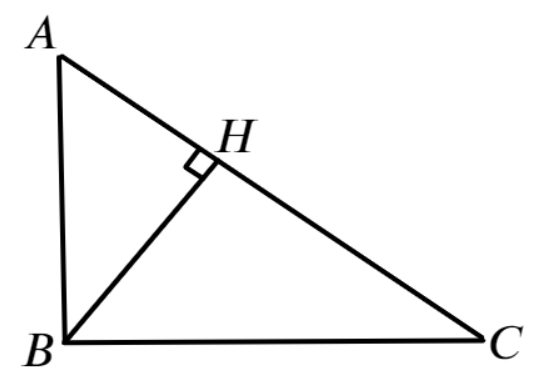
\includegraphics[scale=0.35]{g8-111.png}}
\end{figure}\\
Найдём $\angle A=90^\circ-60^\circ=30^\circ,\ \angle CBH=90^\circ-60^\circ=30^\circ.$ Пусть $CH=x,$ тогда по теореме о прямоугольном треугольнике с углом в $30^\circ$ для треугольников $CBH$ и $ABC$ имеем соотношения $BC=2x,\ AC=2BC=4x.$ Тогда $AC=AH+HC,\ 4x=18+x,\ x=6.$\\
